\chapter{蛋白质复合物特征子图样本生成}
\label{chapter:featSubNetworkConstruct}

本章主要介绍蛋白质复合物特征子图的生成,其中包括蛋白质相互作用网络构建、结点特征生成与嵌入、邻边特征生成与嵌入以及特征子图样本的提取。重点在于本章使用了深度学习方法、网络嵌入方法、多种邻边相似性特征提取方法构建具有丰富特征的蛋白质相互作用网络,并在此基础上构建了特征子图样本数据集,包括正样本数据集、中间样本数据集、负样本数据集、待筛选样本数据集。

\section{引言}
\label{section:featSubNetworkConstruct:intro}

目前公开的已验证蛋白质复合物均为以蛋白质集合表示,每一个蛋白质集合代表一个复合物,表示该集合内若干个蛋白质之间具有一定的相互作用并形成复合物。但是集合的数据不具有可学习性,计算方法无法有效识别某个蛋白质集合能否形成复合物,因此需要将集合数据转换为复合物的结构化数据,结构化数据为从蛋白质复合物特征子图。特征子图中包含了复合物中的蛋白质集合、蛋白质相互作用数据、蛋白质特征以及蛋白质相互作用特征。在蛋白质复合物结构化数据的基础上,深度学习的方法可以有效的挖掘蛋白质复合物的内部规律,学习蛋白质复合物的形成条件。

蛋白质复合物特征子图样本的构造需要以下几步。首先利用已知的蛋白质相互作用数据集构建蛋白质相互作用网络,再在互作网络的基础上嵌入丰富的结点特征和邻边特征,形成带特征的蛋白质相互作用网络,最后根据蛋白质复合物中的蛋白质集合作为子图结点集合从带特征的蛋白质相互作用网络中提取特征子图。按照蛋白质复合物数据来源划分,特征子图可以区分为正样本特征子图、中间样本特征子图、负样本特征子图和待筛选特征子图,前三者作为训练集训练蛋白质复合物筛选模型,最后复合物筛选模型会在待筛选特征子图进行测试。

\section{蛋白质相互作用特征网络构建}
\label{section:featSubNetworkConstruct:featPPINetwork}

蛋白质相互作用特征网络构建目标是将蛋白质的相互作用数据转换为图结构,并为图结构添加结点特征和邻边特征。以下分别介绍图结构的形成、结点特征的添加以及邻边特征的添加。

\subsection{基于互作关系构建蛋白质相互作用网络}
\label{subsection:featPPINetwork:networkConstruct}

酿酒酵母(Saccharomyces cerevisiae)的蛋白质相互作用中有较深入的研究,其标准复合物数据集,蛋白质相互作用数据较为完备,因此本文基于酿酒酵母的蛋白质互作网络展开研究。

本文选取了主流的酿酒酵母细菌的$PPI$数据集,包括DIP\cite{salwinski_database_2004}、Krogan\cite{krogan_global_2006}、Biogrid\cite{stark_biogrid_2006}和Gavin\cite{gavin_proteome_2006}。

DIP数据集是结合各种来源的信息创建的一致的$PPI$数据集,可以自动从论文中提取关系数据并更新数据库,同时有专业人员管理。
Krogan数据集使用$LC_MS/MS$技术检测蛋白质相互作用并借助机器学习方法提高结果的可靠度,数据集分为核心和附属两个部分,本文将核心附属网络融合进行实验。
Biogrid数据集融合了多个数据集来源,同时排出了不符合多重验证标准的相互作用。
Gavin数据集基于亲和纯化与质谱技术检测蛋白质相互作用,并使用socio-affinity指数评估$PPI$检测结果的可靠度。

每个数据集都由若干蛋白质相互作用对组成,表示两个蛋白质之间存在相互作用关系,依据关系数据,可以相应的构造$PIN$。$PIN$以$G=\{V,E\}$的形式存在,$G$为一个图结构(Graph),$V$为图结构的所有结点,每一个结点代表一个蛋白质,$E$为图结构中的所有邻边,每一条邻边代表两个蛋白质之间存在相互作用关系,如$E=\{V_i,V_j\}$代表第i个蛋白质和第j个蛋白质之间存在互作关系。图结构以邻接矩阵的形式存在$A\in \mathbb{R}^{n\times n}$。

数据集具体的网络结构如图\ref{fig:ppi-datasets}所示,具体统计学特征如表\ref{tab:PPIStatic}所示。

\begin{figure}[htbp]
    \centering
    \subcaptionbox{DIP数据集}{\label{fig:ppi:zitu:a}
        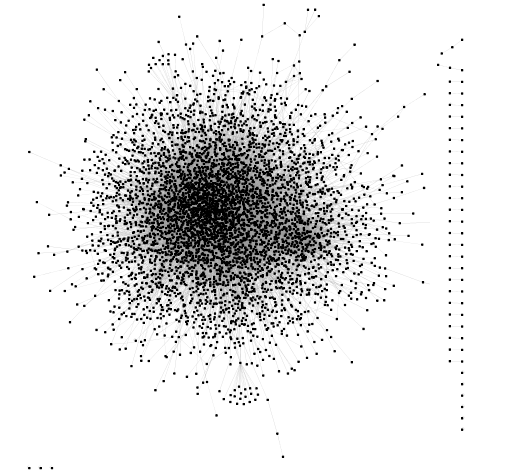
\includegraphics[width=5cm]{PPI/DIP.png}}
    \subcaptionbox{Krogan数据集}{\label{fig:ppi:zitu:b}
        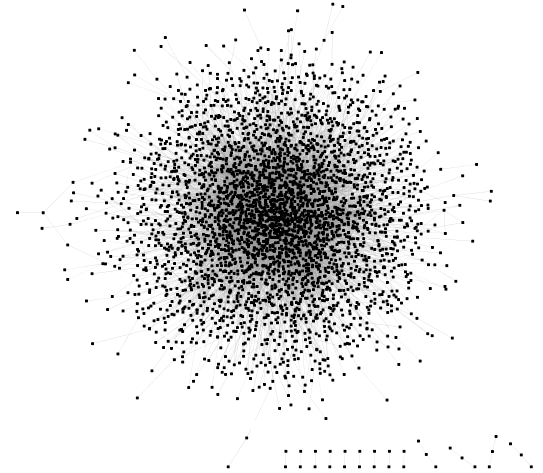
\includegraphics[width=5cm]{PPI/Krogan.png}}
    \vskip0.5cm
    \subcaptionbox{Biogrid数据集}{\label{fig:ppi:zitu:c}
        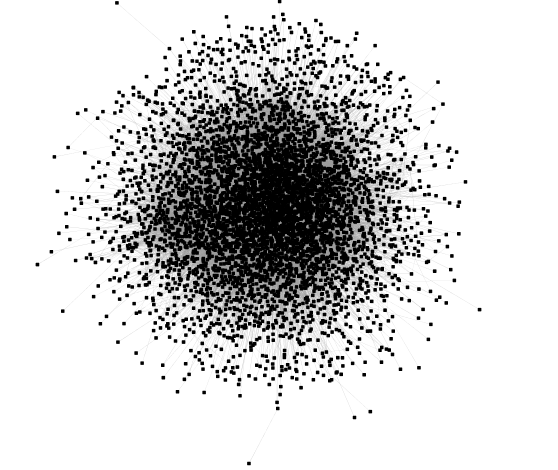
\includegraphics[width=5cm]{PPI/Biogrid.png}}
    \subcaptionbox{Gavin数据集}{\label{fig:ppi:zitu:d}
        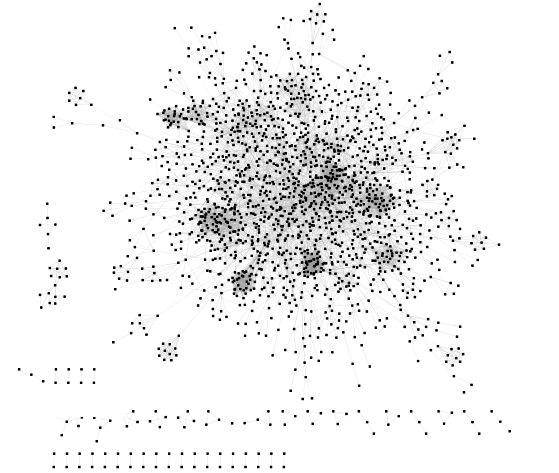
\includegraphics[width=5cm]{PPI/Gavin.png}}
    \caption{蛋白质相互作用数据集}
    \label{fig:ppi-datasets}
\end{figure}


\begin{table}[h]
    \centering
    \caption{$PPI$数据集统计表}
    \label{tab:PPIStatic}
    \begin{tabular}{L{4.2cm}L{2cm}L{2cm}L{2cm}L{2cm}}
        \toprule
        \textbf{网络特征} & \textbf{DIP} & \textbf{Krogan} & \textbf{Biogrid} & \textbf{Gavin} \\
        \midrule
        蛋白质数          & 4928         & 3672            & 5573             & 1855           \\
        相互作用数        & 17201        & 14317           & 59636            & 7669           \\
        平均度数          & 6.98         & 7.80            & 21.40            & 8.27           \\
        密度              & 0.0014       & 0.0021          & 0.0038           & 0.0044         \\
        平均聚类系数      & 0.0945       & 0.1203          & 0.2483           & 0.4674         \\
        连通个数          & 28           & 14              & 1                & 43             \\
        最大连通结点数    & 4873         & 3642            & 5573             & 1727           \\
        传递性            & 0.0728       & 0.1001          & 0.0657           & 0.5676         \\
        直径              & 11           & 10              & 6                & 13             \\
        \bottomrule
    \end{tabular}
\end{table}

从表\ref{tab:PPIStatic}中可以看出,DIP数据集和Biogrid数据集是结点数和邻边数最大的两个数据集,同时其度数差异性较大,本文的研究工作主要围绕这两个数据集展开。最后,本文得出的模型效果也会在Krogan数据集和Gavin数据集进行验证。

利用$PPI$数据集构建相应的$PIN$网络结构之后,可以将蛋白质特征以及蛋白质相互作用特征添加到网络中去,形成带有生物特征的蛋白质相互作用网络$Feated-PIN$。在蛋白质相互作用网络结点上添加蛋白质自有特征和嵌入特征作为结点的初始特征。蛋白质自有特征包括蛋白质序列长度、分子重量特征,蛋白质嵌入特征包括图自编码器器(Graph Auto Encoding,简称GAE)和结点嵌入模型(Node2Vec)中的深度随机游走方法(Deepwalk)得到的图嵌入特征。在蛋白质相互作用网络邻边上添加通过生物计算的蛋白质相互作用特征,包括蛋白质功能注释特征、拓扑域相似性特征和亚细胞定位相似性特征,以及蛋白质拓扑域相似性特征作为图网络里面邻边的初始特征。

下面分别介绍结点特征的嵌入方法和邻边特征的嵌入方法。

\subsection{基于图自编码器器和深度随机游走的结点特征嵌入}
\label{subsection:featPPINetwork:nodeFeatConstruct}

图结构是高维的复杂的数据,包含噪声和冗余信息,直接的图结构数据无法应用于机器学习或数据分析任务中。结点特征嵌入就是将网络数据映射到低维空间中,从而学习到网络节点的低维向量表示,低维向量的长度一般为固定值,远小于网络的结点数量。在低维表示下,可以应用丰富的数据分析方法进行进一步处理,比如结点分类、链路预测、图分类等等。

传统的结点表示方法是基于拓扑的,直接通过邻接矩阵的简单运算得到结点的特征,其中可能包含过量的噪声或冗余信息。

\begin{figure}[htbp]
    \centering
    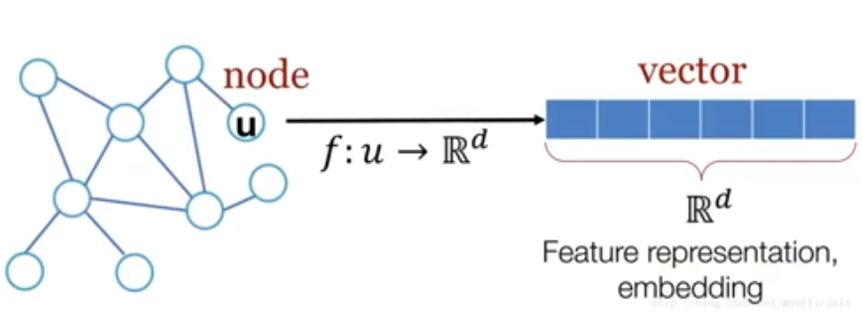
\includegraphics[width=6cm]{node-vec.png}
    \caption{结点特征嵌入示意图}
    \label{fig:node-vec}
\end{figure}

\begin{figure}[htbp]
    \centering
    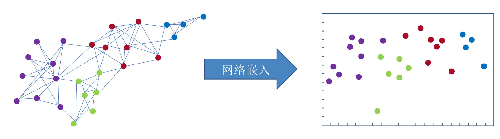
\includegraphics[width=8cm]{node-embedding}
    \caption{结点特征嵌入映射到二维平面示意图}
    \label{fig:node-embedding}
\end{figure}

图\ref{fig:node-vec}展现了结点特征表示的过程,结点u经过特征嵌入后,可以转换为长度为d的向量表示,$\mathbb{R} ^d$向量完全表达了结点信息。图\ref{fig:node-embedding}展现了在结点分类任务上,网络嵌入的分类效果,经过结点嵌入的各个结点可以转换为一系列的向量,将该系列的向量映射到二维空间之后,可以依旧按照原始网络中的分布规律在平面内聚簇分布,如图中不同颜色的聚簇表示。

本文基于图自编码器和深度随机游走嵌入对蛋白质相互作用网络中的蛋白质结点特征进行嵌入,同时在蛋白质结点中保留了部分蛋白质自有的生物学信息嵌入。具体介绍如下所示。

\subsubsection{基于图自编码器的结点特征嵌入}

图自编码器是一种基于深度学习的结点嵌入方法,其核心思想是结点的嵌入特征需要具备有效恢复整个网络结构的信息。在此前提基础上图自编码器主要有两个过程,编码过程和解码过程,编码到解码的中间状态的结点表示即为图中的结点特征嵌入。
图自编码器的编码过程基于图卷积神经网络实现,解码过程基于链路预测和网络还原实现。

下面分别对图卷积神经网络、自编码器以及图自编码器做简单介绍,后续介绍基于图自编码器的蛋白质互作网络结点嵌入模型。

\subparagraph{1)~图卷积神经网络} ~

卷积神经网络快速发展,其具有高效的特征提取能力。相比传统方法,卷积神经网络给图像处理和自然语言处理等领域带来了空间的提升,如机器翻译、图像识别和语音识别等。但是传统的卷积神经网络只能处理欧氏空间数据,欧式空间数据具有平移不变性,其定义的全局共享的卷积核可以处理所有的数据点,如图像数据中,图片转换为像素点,任意像素点为中心都可以按同样的卷积核提取周围的信息。

图结构数据是非欧式空间数据,图数据中每个结点的局部结构各异,这使得图数据不具有平移不变性。图卷积神经网络(Graph Convolution Network,简称GCN)的提出解决了该缺陷,GCN基于邻居特征聚集以及将转换矩阵作为卷积核的思想巧妙的实现了在每一个结点做相同卷积过程。

单个的图卷积过程具体如公式\ref{equ:gcn}所示。
\begin{equation}
    \label{equ:gcn}
    H^{(l+1)}=\sigma (\hat{A}H^{(l)}W^{(l)})
\end{equation}
其中$\hat{A}\in \mathbb{R}^{n\times n} $为经过拉普拉斯平滑的邻接矩阵;$H^{(l)}\in \mathbb{R}^{n\times m} $代表第l层的结点特征矩阵,其中每一个结点特征维度为m;$W^{(l)}\in \mathbb{R}^{m\times m} $代表卷积核,代表每一个结点的特征转换;$\sigma $为激活函数;$H^{(l+1)}\in \mathbb{R}^{n\times m} $代表经过一轮卷积之后的输出结果。

类似于传统的卷积方式,GCN也可以多层卷积组合到一起进行,如图\ref{fig:GCN/main}所示。图卷积的输入为邻接矩阵代表的图结构和特征矩阵代表的结点特征,隐层之间采用Relu的激活函数,最后得到图的结点特征。

\begin{figure}[htbp]
    \centering
    \includegraphics[width=14cm]{GCN/main}
    \caption{GCN示意图}
    \label{fig:GCN/main}
\end{figure}

\subparagraph{2)~自编码器} ~

自编码器(Auto Encoder)是无监督模型,由编码器和解码器两部分构成。编码器的任务是将原始的输入数据转换为编码数据表示,类似于数据压缩数据或者特征提取过程。解码器是将编码器得到的数据重新还原成原始的输入数据。自编码器的训练目标是使最终输出数据和原始输入数据之间的误差尽量小。基于该目标,自编码器的中间层编码数据具有复原输入的能力,可以认为这种编码数据表示有效地提取到了原始数据的特征。通常情况下,编码数据较原始数据维度低,具有一定的数据降维能力,同时也能去除数据中的噪声,有效提高数据的可用性。

\begin{figure}[htbp]
    \centering
    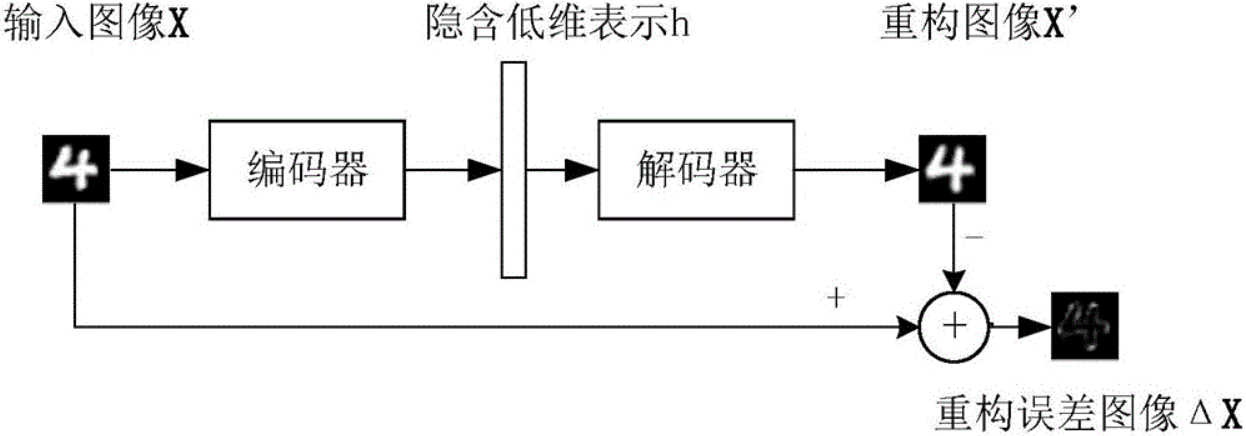
\includegraphics[width=9cm]{gae/autoencoder}
    \caption{自编码器示意图}
    \label{fig:gae/autoencoder}
\end{figure}

图\ref{fig:gae/autoencoder}为经典的图片自编码器示意图,输入图像为$X$,中间编码为$h$,输出图像为$X^\prime $,输入输出差距为$\varDelta X$,编码器的函数过程可以用$F$表示,解码器过的函数过程可以用$G$表示。总体过程可以如式\ref{equ:autoencoder}所示。通过反向传播不断的减小$\varDelta X$,最终隐层编码表示即可学习到输入图像的特征。
\begin{equation}
    \label{equ:autoencoder}
    X^\prime =G(F(X)),
    \varDelta X={\| X^\prime - X \Vert}
\end{equation}

\subparagraph{3)~图自编码器} ~

图自编码器是结合了图卷积神经网络和自编码器的一种用于处理图结构数据的深度神经网络。其具体过程如图\ref{fig:gae/main}表示,其目标是对图结构进行编码,得到结点的特征表示。

相较于普通的自编码器,图自编码器的输入为图的邻接矩阵$A$和图的特征矩阵$H$,编码过程是多层的图卷积神经网络,解码过程是用编码之后的结点特征做基于相似性计算的链路预测,最终对比经过链路预测得到的邻接矩阵$A^{\prime}$和输入的邻接矩阵$A$的差异。

\begin{figure}[htbp]
    \centering
    \includegraphics[width=14cm]{gae/main}
    \caption{GAE示意图}
    \label{fig:gae/main}
\end{figure}


\subparagraph{4)~基于图自编码器的蛋白质互作网络结点嵌入模型} ~

本节介绍在蛋白质互作网络上基于图自编码器的结点嵌入模型。

本文的自编码器模型的初始输入特征为常数,本文设定为1,这种情况会削弱输入结点特征对模型的影响,使模型能够关注并学习到相互作用网络的全局的拓扑特征。

编码过程采用3层GCN网络,第一层GCN网络的特征转换矩阵为$\mathbb{R} ^{1\times 64}$,第二层GCn网络的特征转换矩阵为$\mathbb{R} ^{64\times 64}$,第三层GCn网络的特征转换矩阵为$\mathbb{R} ^{64\times 16}$,即最终得到的结点隐层表示维度为16维,整个网络中结点的隐层特征为$\mathbb{R} ^{n\times 16}$。
采用三层GCN网络可以使得结点可以获取3跳之外的邻居信息,通过GCN融合到一起就可以整个直径范围为7的信息,通过\ref{tab:PPIStatic}的统计可以得出,不同的$PIN$的全局图直径在6~12,因此这个卷积方法可以融合至少半个图结构范围的信息,一定程度上可以体现结点的全局拓扑特征。
在每层GCN中,模型采用了Relu函数作为激活函数,同时模型采用了全局0.1的Dropout,一定程度上防止模型的过拟合。

\begin{figure}[htbp]
    \centering
    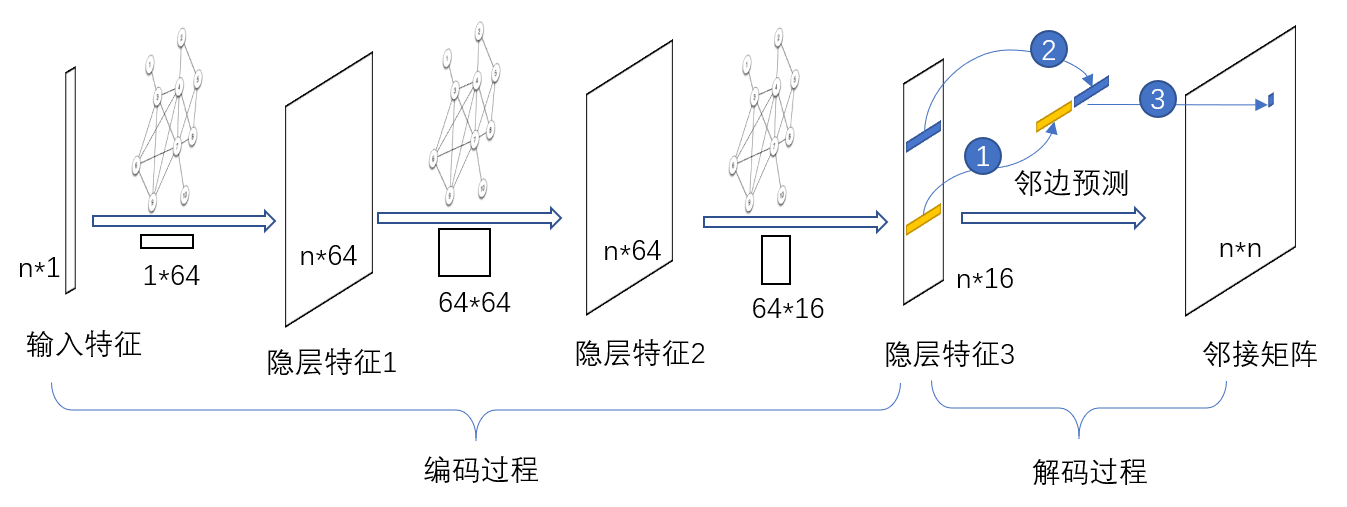
\includegraphics[width=15cm]{gae/mygae}
    \caption{基于图自编码器的蛋白质互作网络结点嵌入模型}
    \label{fig:gae/mygae}
\end{figure}

解码过程采用了基于神经网络的链路预测模型,对于图中的每一条可能的邻边,基于邻边两个端点的特征组合到一起,经过两层神经网络,再经过Softmax激活函数得到一个0至1的数值,代表该条邻边存在的可能性,具体过程如式\ref{equ:decoder}所示。

\begin{equation}
    \label{equ:decoder}
    E_{i,j} =softmax(f(cat(H_i,H_j)))
\end{equation}

式中$H_i$和$H_j$为经过编码器编码的结点i和j的特征,$E_{i,j}$为邻边存在的概率。最终预测得到的图邻接矩阵为$A^{\prime}$。


损失函数为预测的$PIN$邻接矩阵$A^{\prime}$和真实邻接矩阵$A$的MSELoss(Mean Square Error Loss)。

\begin{equation}
    \label{equ:autoembedloss}
    \quad l_n =\frac{\sum_{e_{ij}\in G}{  \left( A_{ij}^{\prime} - A_{ij} \right)^2}}{n^2}
\end{equation}
其中G代表图结构,$e_{ij}$代表图结构中i结点和j结点连边,而$A_{ij}^{\prime}$为预测的边权重,$A_{ij}$为原始图中真实的边权重,如果原始图中邻边不存在,权重为0。


训练过程的其他训练细节如下所示。训练过程中采用了Adam优化器,学习率为0.01,模型训练轮数为80epoch。

最终基于图自编码器的蛋白质互作网络结点嵌入模型采用最后一轮的隐层作为最终的结点嵌入,最终的结点嵌入结果为$\mathbb{R}^{n\times 16}$的特征矩阵。

具体算法如下所示。
\begin{algorithm}[h]
    \caption{Graph Auto-Embedding in PIN} % 名称
    \label{alg::gae}
    \begin{algorithmic}
        \Require
        $G$: PIN graph struct data;
        $A$: adjacent matrix of $G$;
        $i$: epoch index;
        $Dec$: Multi-layer perceptifier;
        \Ensure
        $F$: $\mathbb{R}^{n\times 16}$ node feat after GAE Process;
        \State initial nodefeat=1, $F_0$;initial i=0;
        \Repeat
        \State compute hidden feat 1, $F_1=GCN(G,F_0)$;
        \State compute hidden feat 2, $F_2=GCN(G,F_1)$;
        \State compute hidden feat 3, $F_3=GCN(G,F_1)$;
        \State reconstruct graph, $A^{\prime}=Dec(F_3)$;
        \State compute loss, $L=MSELoss(A^{\prime},A)$;
        \State optimization, $Adam(L)$;
        \State i=i+1;
        \Until{$i=80$}
        \State extract node feats to $F$, $F$=$F_3$;
    \end{algorithmic}
\end{algorithm}

\subsubsection{基于Deepwalk的结点特征嵌入}

Deepwalk是基于随机游走的图结点嵌入模型,基本思想是通过在图中随机游走的方式获取若干结点的序列,这些序列被当作具有上下文语言的语句,而结点被当作语句中的一个单词。通过Word2Vec的模型,将语句中的单词转换为向量,作为结点的特征,即可得到结点特性嵌入。在图中游走获取的结点序列能够在一定程序上包含结点周围的拓扑信息,若干周围信息组合到一起则可以提取出整个图结构的拓扑信息。通过序列获取结点嵌入后使结点依旧保持图结构的拓扑信息。

RandomWalk是一种可重复访问已访问节点的深度优先遍历算法。给定当前访问起始节点,从其邻居中随机采样节点作为下一个访问节点,重复此过程,直到访问序列长度满足预设条件。该采样过程得到的序列如图\ref{fig:deepwalk/main}中的b部分所示。

Skip-gram是一种词向量嵌入模型,基本思路是利用序列中的单个词预测周围词的模型,在学习了所有序列之后,可以得到每一个结点的特征嵌入。利用Skip-gram模型获取结点的嵌入过程如图\ref{fig:deepwalk/main}中的c部分所示。

\begin{figure}[htbp]
    \centering
    \includegraphics[width=10cm]{deepwalk/main}
    \caption{deepwalk嵌入示意图示意图}
    \label{fig:deepwalk/main}
\end{figure}

考虑到$PIN$的规模,本文的Deepwalk嵌入模型的序列长度为100,基于每一个结点均随机游走采用10跳序列,最终的序列数据为$10n*100$,n为不同的$PIN$的结点数。最终获取的Deepwalk嵌入特征维度为64维。

\subsubsection{基于蛋白质自有特征的结点特征嵌入}

在细胞中,蛋白质可以由一系列氨基酸构成,基于氨基酸序列本文获取了部分蛋白质特征,分别为氨基酸序列的长度和蛋白质的重量。

其中氨基酸长度可以代表由氨基酸生成该蛋白质的困难程度,需要多少个氨基酸才能组合成该蛋白质。而蛋白质的重量一定程度上反映了生成该蛋白质消耗的元素量,体现了蛋白质重要程度。本文采用了蛋白质的序列长度和质量两项特征作为蛋白质的自有特征。

\subsubsection{结点特征嵌入汇总}
在结点特征嵌入阶段,计算了$PIN$中蛋白质的GAE嵌入特征、Deepwalk嵌入特征以及蛋白质的自有特征。$PIN$中每个结点特征嵌入维度为82维,其计算公式如\ref{equ:feat:nodecat}所示,具体分布如表\ref{tab:PINedgeFeatNums}所示:
\begin{equation}
    \label{equ:feat:nodecat}
    F_i=Concat(F_i^{GAE},F_i^{Deepwalk},F_i^{Self})
\end{equation}
其中$i$表示第i个结点,$Concat$为特征拼接函数,$F_i$为第i个结点融合之后的82维特征,$F_i^{GAE}$为基于GAE得到的16维结点特征,$F_i^{Deepwalk}$为基于Deepwalk得到的64维结点特征,$F_i^{Self}$为基于蛋白质自有数据得到的2维结点特征。

\begin{table}[h]
    \centering
    \caption{$PIN$结点特征维度分布}
    \label{tab:PINNodeFeatNums}
    \begin{tabular}{C{3cm}C{5cm}C{3cm}}
        \toprule
        \textbf{GAE嵌入特征} & \textbf{Deepwalk嵌入特征} & \textbf{结点自有特征} \\
        \midrule
        16                   & 64                        & 2                     \\
        \bottomrule
    \end{tabular}
\end{table}

\subsection{基于多种相似性计算方法的邻边特征嵌入}
\label{subsection:featPPINetwork:edgeFeatConstruct}

除了蛋白质的结点特征,蛋白质之间也存在复杂的相互所有关系,不同的相互作用关系由于作用的蛋白质结构域不同、功能不同、发生作用的生理位置不同等,具有很大的差异性。在一般的方法中,这部分差异性仅仅映射在作用强度一个单一的数值中,在本文中,将这种丰富的作用差异作为邻边的特征完整的嵌入到图结构中,如图\ref{fig:edgefeat/main}所示。


\begin{figure}[htbp]
    \centering
    \includegraphics[width=10cm]{edgefeat/main}
    \caption{edgefeat嵌入示意图}
    \label{fig:edgefeat/main}
\end{figure}
本文为蛋白质相互作用网络的所有邻边嵌入相同维度的特征,特征中相同标号的数据具有同样的生物学意义。本文为邻边嵌入的特征包括基于蛋白质GO功能注释相似性的特征、基于蛋白质拓扑域相似性特征、基于蛋白质亚细胞定位相似性的特征和基于拓扑相似性的特征。下面分别介绍这四类相似性特征。

\subsubsection{蛋白质GO功能注释相似性的邻边特征嵌入}

基因本体信息\cite{ashburner_gene_2000}即GO注释信息是描述蛋白质功能表达的词汇表,将生物活动过程进行统一编码表示,其在生物信息学领域得到了广泛的应用。对应到蛋白质中,蛋白质分子参与的若干生物过程均可对应到GO注释表,形成对该蛋白质的综合功能描述。GO注释项总体分为三类,分别是生物过程(Biological Process)、分子功能(Molecular Function)及细胞组成(Cellular Component),生物过程描述分子功能有序组成的生命活动,分子功能描述分子在生物学上的活性,细胞组成描述了亚细胞结构及位置信息。GO注释项之间由于描述涵盖范围的不同,具有一定的从属关系,所有的GO注释项可以组成有向无环图(Directed Acyclic Graph,简称DAG)。图\ref{fig:go-dag}为QuickGO\cite{binns_quickgo_2009}网站中获取的生殖细胞发育过程对应的GO注释DAG图。GO注释信息的从属关系主要分为两种,分别是$is\_a$和$part\_of$,其中$is\_a$表示包含关系,如图中黑色箭头所示,$part\_of$表示从属关系,如图中蓝色箭头所示。图中每一个方框展示了GO注释项及其生物功能。
\begin{figure}[htbp]
    \centering
    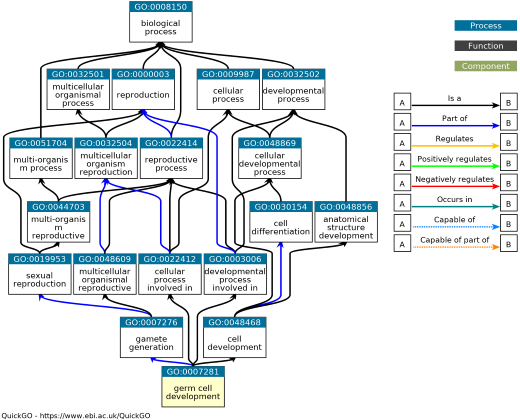
\includegraphics{go-dag}
    \caption{生殖细胞发育对应的GO示意图}
    \label{fig:go-dag}
\end{figure}

通常情况下,蛋白质复合物中蛋白质倾向于相同的功能表达,同时功能表达相似性越高时,蛋白质产生相互作用的可能性越大。部分算法\cite{ulitsky_identification_2007,jianxing_feng_max-flow-based_2011}基于功能表达数据提出了$PIN$连边权重更新的方法。
本文采用两种方法计算蛋白质功能相似度,将计算结果作为$PIN$网络中邻边的蛋白质功能特征。

\subparagraph*{基于DAG图的GO相似性计算}

本方法参考了Wang等人\cite{wang_new_2007}提出的方法,给定一个GO注释项$p$,从GO的总体DAG图中提取子图$DAG_p(A,T_p,E_p)$,其中$T_p$是$p$及所有$p$的祖先结点的注释项,$E_p$表示所有截取的注释项的连接关系。
定义$T_p$中每一个结点对$p$的语义值如下:
\begin{equation}
    \label{equ:feat:go:SAT}
    S_p(t)=\left\{\begin{array}{l}
        1,t=p                                                                        \\
        \max {\{ w_e\times S_p(t^\prime )| t^\prime\in ~children~of~(t) \} },t\neq p \\
    \end{array}\right.
\end{equation}
其中$w_e$是$t^\prime$和$t$之间的权重,定义两种类型的边$is\_a$和$part\_of$权重各自为0.8和0.6。有公式可以直观得出,祖先结点点中离$p$注释越远的注释项,其对$p$的语义值越小,而$p$对自身的语义值贡献为1。
定义了所有祖先结点对$p$的语义值之后,可以直接得出$p$的语义值得分,计算公式如下:
\begin{equation}
    \label{equ:feat:go:SVA}
    SV(p)=\sum_{t \in T_p}(t)
\end{equation}
按照该计算方法,可以得到每一个注释项各自的语义值,在此基础上可以得到两个注释项$p$,$q$语义值的相似度,具体计算方法如下:
\begin{equation}
    \label{equ:feat:go:SimItemWang}
    WSim_{GO}(p,q)=\frac{\sum_{t \in T_p \cap T_q}(S_p(t)+S_q(t))}{SV(p)+SV(q)}
\end{equation}
其中$t$为$p$和$q$的所有公共祖先结点。由于蛋白质通常是由多个注释项组成,因此蛋白质之间的功能相似性需要考虑两个蛋白质各自注释项之间的综合结果,其具体计算方法如下:
\begin{equation}
    \label{equ:feat:go:SimProteinWang}
    \begin{aligned}
        WSim_{Protein}(P,Q) & =\frac{1}{m+n}\cdot \left\{\sum_{1\leq i\leq m}{\max_{1\leq j\leq n}[{Sim_{GO}(p_i,q_j)}}]\right. \\
                            & \left.+\sum_{1\leq j\leq n}{\max_{1\leq i\leq m}[{Sim_{GO}(p_i,q_j)}}]\right\}
    \end{aligned}
\end{equation}
其中$P$,$Q$表示两个蛋白质,其中分别具有$\{p_i| i=1,2,\dots,m\}$,$\{q_j| j=1,2,\dots,n\}$的功能注释项。
这个方法的核心思想是将两个蛋白质的注释信息相互关系矩阵$m\times n$构造出来,只考虑源蛋白质的某一个注释项和目标蛋白质所有注释项最大的相关性,而蛋白质的相互作用关系是所有最大值的平均。

\subparagraph*{基于频率统计的GO相似性计算}

本方法参考了Lin等人\cite{lin_information-theoretic_1998}提出的方法。首先计算某两个注释项之间的相关性,具体计算过程如下:
\begin{equation}
    \label{equ:feat:go:SimItemLin}
    LSim_{GO}(p,q)=\min_{anc \in Ancient(p,q)}\mathcal{P} (anc)
    % Sim_{GO}(p,q)=\max{\frac{2\times \log }{} }
\end{equation}
其中$Ancient(p,q)$表示两个注释项的公共祖先,而$\mathcal{P}$表示某一个注释项在所有蛋白质中出现的概率。这个计算公式直观的认为,两个具有相互关联的功能注释,其关联结点越稀有,则表示两个注释项的相关性越强。计算蛋白质功能相似性的计算方法如下:
\begin{equation}
    \label{equ:feat:go:SimProteinLin}
    LSim_{Protein}(P,Q)=\max{\frac{2\times \log \{Sim_{GO}(p,q)\}}{\log {\mathcal{P}_p}+\log {\mathcal{P}_q}} }
\end{equation}

\subsubsection{蛋白质结构域相似性的邻边特征嵌入}

蛋白质结构域时蛋白质具有独立功能和特异结构的区域,结构域互作信息影响蛋白质复合物的形成\cite{kim_relating_2006}。结构域之间具有相互作用关系,这些相互作用关系可以从三维交互域(3did)数据库\cite{mosca_3did_2014}提取,并构建成结构域相互作用网络(Domain-Domain Interaction Network,简称DDI)。
单个蛋白质所具有的结构域可以映射到结构域互作网络的若干结点,成为一个结构域集群,而蛋白质域相似性可以转换为两个结构域集群的相互作用关系。
本文中两个蛋白质的结构域互作特征包括如下方面:两个蛋白质结构域交集、并集以及相互之间的差集;映射到结构域相互网络之后,两个结构域集群之间的相互作用关系数量,其具体的计算公式如下:
\begin{equation}
    \label{equ:feat:domain}
    Sim_{domain} = \sum_{i \in dom(p)}{\sum_{j \in dom(q)}{Weight_{ij}}}
\end{equation}
其中$i$、$j$分别时蛋白质$p$、$q$之间的结构域,$Weight_{ij}$代表结构域$i$、$j$在结构域相互作用网络中的作用强度,对于无权网络可以取值为1。

Huang等人\cite{huang_protein-protein_2013}在运用结构域相互作用网络预测蛋白质相互作用时,提出了使用一阶邻居和二阶邻居计算$domain$相似性的想法,其扩展方式如图\ref{fig:domain-second}所示。本文也同时补充了一阶和二阶扩展之后的蛋白质$domain$相似性特征。
\begin{figure}[htbp]
    \centering
    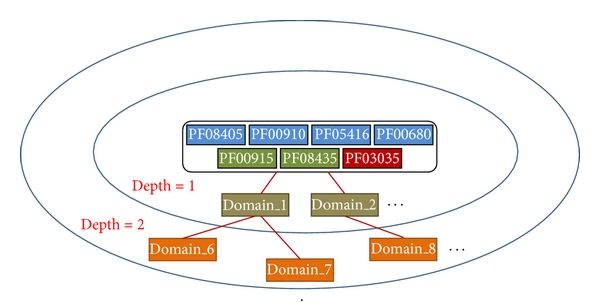
\includegraphics[width=8cm]{domain-second}
    \caption{DDI多阶邻居示意图}
    \label{fig:domain-second}
\end{figure}

\subsubsection{蛋白质亚细胞定位相似性的邻边特征嵌入}

细胞是一个高度有序的结构,胞内根据空间分布和功能不同,可以分成不同细胞器或细胞区域,蛋白质只有转运到正确的部位才能参与细胞的各种生命活动,ZHANG等人\cite{zhang_protein_2007}认为蛋白质的亚细胞定位有助于研究蛋白质的生物学功能,同时对蛋白质的其他研究如相互作用、进化等也能提供必要的信息。Huang等人提出\cite{fan_genome-wide_2017}使用蛋白质复合物和亚细胞定位信息预测关键蛋白质,蛋白质复合物,蛋白质复合物的生成和功能实现和其所处的细胞位置相关,因此蛋白质的亚细胞定位能对蛋白质复合物的形成产生一定的影响。本文将两个蛋白质亚细胞定位数据的交集和并集作为蛋白质的亚细胞定位特征。图\ref{fig:subcell}为苏氨酸蛋白激酶TOR1亚细胞定位图,其中黄色的部分表示其主要的注释区域,包括细胞膜和液膜。

\begin{figure}[htbp]
    \centering
    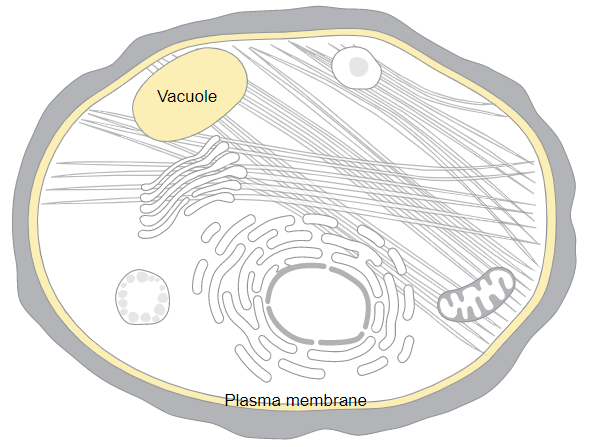
\includegraphics[width=8cm]{subcell}
    \caption{苏氨酸蛋白激酶TOR1亚细胞定位图}
    \label{fig:subcell}
\end{figure}

\subsubsection{蛋白质拓扑相似性的邻边特征嵌入}

蛋白质在$PIN$中所处的拓扑环境也可以作为蛋白质相似性特征的计算方式。基于DPClus算法\cite{altaf-ul-amin_development_2006}中提出的相似性计算方法,本文将结点的公共邻居数作为拓扑相似性特征。具体计算方法如下:
\begin{equation}
    \label{equ:feat:topoCN}
    CN_{(P,Q)} = \left\lvert N_P\cap N_Q\right\rvert
\end{equation}
其中$P$,$Q$为相互作用的蛋白质,$N_P$和$N_Q$分别为两个蛋白质在$PIN$中的邻居。

\subsubsection{邻边特征嵌入汇总}

在邻边特征嵌入阶段,计算了$PIN$中所有蛋白质相互作用之间的相似性特征,其中包括蛋白质功能注释特征、结构域特征、亚细胞定位特征以及网络拓扑特征。$PIN$中每条相互作用边所具有的特征维度为12维,具体计算如公式\ref{equ:feat:edgecat}所示,具体分布如表\ref{tab:PINedgeFeatNums}所示:

\begin{equation}
    \label{equ:feat:edgecat}
    F_{ij}=Concat(F_{ij}^{GO},F_{ij}^{DDI},F_{ij}^{Subcell},F_{ij}^{Topo})
\end{equation}
其中${ij}$表示第i个结点和第j个结点之间的邻边,$Concat$为特征拼接函数,$F_{ij}$为邻边ij融合之后的12维特征,$F_{ij}^{GO}$为基于功能注释相似性得到的2维邻边特征,$F_{ij}^{DDI}$为基于结构域相似性得到的7维邻边特征,$F_{ij}^{Subcell}$为基于亚细胞定位相似性得到的2维邻边特征,$F_{ij}^{Topo}$为一阶邻居相似性得到的1维邻边特征。

\begin{table}[h]
    \centering
    \caption{$PIN$邻边特征维度分布}
    \label{tab:PINedgeFeatNums}
    \begin{tabular}{C{3cm}C{3cm}C{3cm}C{3cm}}
        \toprule
        \textbf{功能注释特征} & \textbf{结构域特征} & \textbf{亚细胞定位特征} & \textbf{网络拓扑特征} \\
        \midrule
        2                     & 7                   & 2                       & 1                     \\
        \bottomrule
    \end{tabular}
\end{table}


\subsection{融合结点特征和邻边特征的蛋白质相互作用网络构建}
\label{subsection:featPPINetwork:addFeat}

通过蛋白质相互作用数据集构造蛋白质相互作用网络,再在网络的基础上应用多种结点嵌入方法和邻边嵌入方法为网络添加结点特征和邻边特征,其工程如图\ref{fig:featedgraph}所示,其中的小矩形代表某一个元素的特征向量,橘色为结点特征向量,蓝色的邻边特征向量。结点总特征维度为82维,邻边总特征维度为12维。

\begin{figure}[htbp]
    \centering
    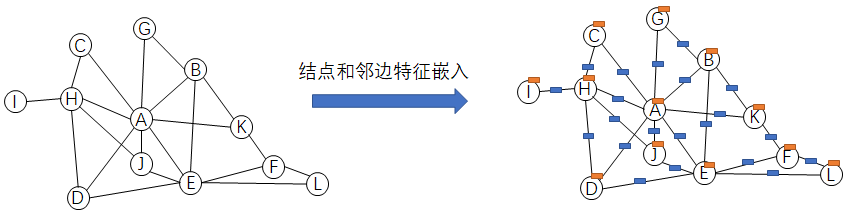
\includegraphics[width=14cm]{featedgraph}
    \caption{结点和邻边特征嵌入示意图}
    \label{fig:featedgraph}
\end{figure}


\section{训练和待筛选复合物特征子图样本生成}
\label{section:featSubNetworkConstruct:allSample}

在具有结点特征和邻边特征的蛋白质相互作用网络($Feated-PIN$)的基础上,按照复合物的对应结点抽取蛋白质复合物特征子图($Feated-subGraph$),该局部图包含了复合物内部蛋白质之间的相互作用关系、相关性特征数据及部分蛋白质特征数据,因此可以将局部图作为后续复合物筛选模型的输入数据。该局部子图的示意图如下所示。

\begin{figure}[htbp]
    \centering
    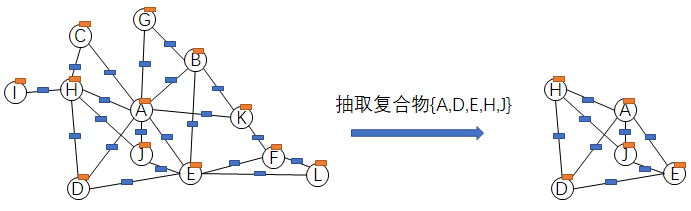
\includegraphics[width=14cm]{extract}
    \caption{复合物子图样本的构造示意图}
    \label{fig:extract}
\end{figure}
在图中,左侧为整个蛋白质相互作用网络,结点$\{A,D,E,H,J\}$为某一个蛋白质复合物的蛋白质集合对应的结点,在获取局部子图的过程中,首先保留结点集合$\{A,D,E,H,J\}$及其结点特征,然后保留结点集合之中的相互作用关系,如邻边$H,J$等。最后形成蛋白质复合物对应的具有结点特征和邻边特征的子图。

本文正样本由酵母菌标准复合物数据集CYC2008\cite{pu_up--date_2009}和MIPS\cite{pagel_mips_2005}构成,负样本为$PIN$上在一定限制条件下产生的随机子图。COACH算法\cite{leung_predicting_2009}作为在复合物预测方法中具有一定准确度和鲁棒性的方法,其产生的样本作为中间样本。待筛选样本为Dpclus算法、Clique算法和IPCA算法在蛋白质复合物网络中的预测结果对应的样本。


\subsection{正样本数据:基于已知蛋白质复合物融合生成}
\label{subsection:allSample:positiveSampleData}

蛋白质复合物数据集通常是由单独的研究机构或学校维护,会每隔一段时间更新生物学上已发现的蛋白质复合物。其中CYC2008数据集和MIPS数据集是针对酿酒酵母的蛋白质复合物数据集,且蛋白质复合物数量较多,更新较快,因此本文采用了CYC2008和MIPS数据集作为标准数据集。

为了训练统一的能够识别真正蛋白质复合物的模型,需要将已知的蛋白质复合物做融合,成为统一的正样本数据。由于不同的正样本数据集可能产生高度相似甚至相同的蛋白质复合物,为了保证样本的独立性,本文做了冗余数据的剔除处理。

本文以此对比了每一对蛋白质复合物并计算其邻居相似性,邻居相似性的计算方法如公式\ref{equ:compComplexSim:NA}所示,邻居相似性代表了两个蛋白质复合物的重合程度。参考已有方法,当两个复合物邻居相似性高于0.8时,本文剔除其中结点数较低的复合物,从而保证最终的正样本集合中无相似样本,具有一定的独立性。最终形成了734个样本的蛋白质复合物数据集。

\begin{equation}
    \label{equ:compComplexSim:NA}
    NA_{(\mathcal{P} ,\mathcal{Q} )} = \frac{{\left\lvert V_{\mathcal{P}} \cap V_{\mathcal{Q}}\right\rvert}^2 }{{\left\lvert V_{\mathcal{P}} \right\rvert}\cdot  {\left\lvert V_{\mathcal{Q}} \right\rvert}}
\end{equation}
其中$\mathcal{P}=(V_{\mathcal{P}} ,E_{\mathcal{P}})$和$\mathcal{Q}=(V_{\mathcal{Q}} ,E_{\mathcal{Q}})$是均表示蛋白质复合物,$V_{\mathcal{P}}$为复合物中的结点集合,$E_{\mathcal{P}}$为复合物中的相互作用集合。

在PPI网络中,由于标准复合物数据集和复合物相互作用数据集可能存在不一致性,部分结点标准复合物数据集存在而互作网络中不存在,为了保证标准复合物的准确性,在抽取子图的过程中,本文会舍弃其中映射到$PIN$网络中出现结点缺失的复合物。

经过上述操作,为在Biogrid网络中剔除结点缺失的样本之后最终的正样本子图数据个数为621个,在DIP网络中剔除结点缺失的样本之后最终的正样本子图数据个数为371个。

\subsection{中间样本数据:基于COACH算法生成}
\label{subsection:allSample:middleSampleData}

COACH算法是一种基于密集子图发现的蛋白质复合物预测算法,可以直接在无权$PIN$网络中预测的蛋白质复合物样本。该方法算法性能优良,且在多个已知的相互作用网络数据集中预测之后,预测结果的召回率和准确率均有较高的数值,其预测的复合物具有一定的指导性,因此本文将COACH算法的预测结果作为独立的中间样本数据。中间样本数据对标准复合物和随机复合物具有一定的区分度,能对分类器识别复合物具有指导作用。

一般情况下,通常复合物预测算法无法无法得到和标准集中的复合物完全重合的结果。当预测的某一个复合物其和标准复合物的最大邻居相似性大于0.25时就认为复合物预测成功。

依据基于邻居相似性的分类标准,COACH生成的样本中有部分复合物预测成功,剩余的复合物预测失败,本文对分类模型的要求时可以区分这两类样本。在可区分该两类样本的情况下,模型对其他算法产生的结果进行筛选时,才可以正确的定位到其中预测成功的样本。因此本文将COACH生成的样本分为两类。
由于邻居相似性处于0.25附近时,样本可能具有较大的迷惑性,反而影响模型的正常训练,因此剔除相似性在0.25附近的部分样本。

本文对中间样本具体做如下处理:
\begin{itemize}
    \item 计算各个样本和标准复合物的最高邻居相似性,得到0$\thicksim$1的分数;
    \item 剔除其中相似性分数高于0.8的样本,防止样本与标准集重合;
    \item 将相似性分数在0.4$\thicksim$1的样本作为A样本;
    \item 将相似性分数在0$\thicksim$0.2的样本作为B样本;
\end{itemize}

经过上述处理,分别得到Biogrid网络和DIP网络运行COACH算法的中间样本数据集,其中Biogrid的A样本为192个、B样本为975个,DIP的A样本为179个、B样本为345个。

\subsection{负样本数据:基于权重动态随机密集子图生成}
\label{subsection:allSample:negtiveSampleData}


随机符合物是在互作网络中随机游走产生的随机图,结合标准样本和中间样本具有紧密型子图的特点,本文对随机游走算法做了一定限制。

首先按照图结点的权重选取初始结点,视作子图。对子图周围所有邻居结点设置权重,邻居结点与子图连接数越高,则该邻居结点权重越高。按照邻居结点权重加权随机抽取下一个结点,并将该结点加入子图,如此反复进行直至子图结点个数达到阈值。按照该种随机子图生成方法,子图趋向于密集连接。由于负样本在子图结构上和正样本相近,在进行分类任务时,可以避免模型学习简单的拓扑差异,迫使模型学习复合物内在的形成规律,达到主动学习的目的。图\ref{fig:diffrent-random-garphs}在DIP网络中采用不同随机算法得到的随机子图差异。

\begin{figure}[htbp]
    \centering
    \subcaptionbox{完全随机子图生成样本1}{\label{fig:randomgraph:zitu:a}
        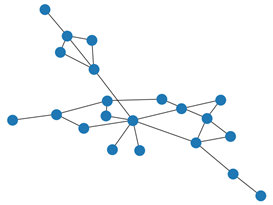
\includegraphics[width=5cm]{randomgraph-old-1}\hskip2cm}
    \subcaptionbox{完全随机子图生成样本2}{\label{fig:randomgraph:zitu:b}
        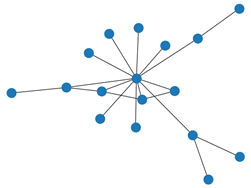
\includegraphics[width=5cm]{randomgraph-old-2}}
    \vskip0.5cm
    \subcaptionbox{限制性随机子图生成样本1}{\label{fig:randomgraph:zitu:c}
        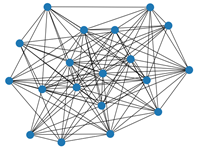
\includegraphics[width=5cm]{randomgraph-new-1}\hskip2cm}
    \subcaptionbox{限制性随机子图生成样本2}{\label{fig:randomgraph:zitu:d}
        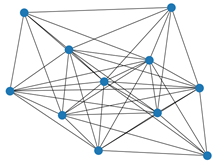
\includegraphics[width=5cm]{randomgraph-new-2}}
    \caption{不同随机算法获取的负样本差异图}
    \label{fig:diffrent-random-garphs}
\end{figure}


本文在网络中按照真实样本的结点数分布抽取负样本,负样本个数为标准样本和中间样本之和。

\subsection{待筛选样本数据:基于核心附属复合物预测算法生成}
\label{subsection:allSample:coreAttachSampleData}

待筛选样本是用于测试模型有效性的测试样本,由已有的复合物预测算法产生。本文采用了基于核心附属的蛋白质复合物预测算法,包括Dpclus算法、Clique算法和IPCA算法,该类算法均具有较高的复合物样本产生量,其召回率的评价指标较高,具有较高的可优化空间。

分别在DIP和Biogrid蛋白质相互作用网络中使用运行复合物预测算法,其得到的预测结果统计如数据汇总与分析所示。




\subsection{数据汇总与分析}
\label{subsection:allSample:summary}

最终产生的训练数据集如下表所示:

\begin{table}[h]
    \centering
    \caption{训练数据集分布统计表}
    \label{tab:datasets:statistic:train}
    \begin{tabular}{C{3cm}C{2cm}C{3cm}C{3cm}C{2cm}}
        \toprule
        \textbf{网络} & \textbf{正样本数} & \textbf{中间样本数(A)} & \textbf{中间样本数(B)} & \textbf{负样本数} \\
        \midrule
        Krogan数据集  & 621               & 192                      & 975                      & 819               \\
        DIP数据集     & 371               & 179                      & 345                      & 764               \\
        \bottomrule
    \end{tabular}
\end{table}

最终产生的待筛选数据集如下表所示:

\begin{table}[h]
    \centering
    \caption{待筛选数据集分布统计表}
    \label{tab:datasets:statistic:beselect}
    \begin{tabular}{C{3cm}C{2cm}C{3cm}C{3cm}C{2cm}}
        \toprule
        \textbf{网络} & \textbf{Dpclus算法} & \textbf{Clique算法} & \textbf{IPCA算法} \\
        \midrule
        Krogan数据集  & 1178                & 3224                & 840               \\
        DIP数据集     & 1078                & 6250                & 438               \\
        \bottomrule
    \end{tabular}
\end{table}


\section{本章小结}
\label{section:FeatSubNetworkConstruct:summary}

本章主要介绍了蛋白质复合物特征子图的生成过程,主要分为两个阶段完成了这个过程。第一阶段是特征蛋白质相互作用网络的构建,其中包括蛋白质相互作用网络构建、结点特征生成与嵌入、邻边特征生成与嵌入。介绍了Deepwalk和GAE为基础的结点特征嵌入方法、介绍了多种基于蛋白质相似性的邻边特征嵌入方法。后续阐述了如何在特征蛋白质相互作用网络基础上上构建了特征子图样本数据集。
